\clearpage

\lehead[]{\sf\hspace*{-2.00cm}\textcolor{white}{\colorbox{lightblue}{\parbox[c][0.70cm][b]{1.60cm}{
\makebox[1.60cm][r]{\thechapter}\\ \makebox[1.60cm][r]{ÜBUNG}}}}\hspace{0.17cm}\textcolor{lightblue}{\chaptertitle}}
\rohead[]{\textcolor{lightblue}{\chaptertitle}\sf\hspace*{0.17cm}\textcolor{white}{\colorbox{lightblue}{\parbox[c][0.70cm][b]{1.60cm}{\thechapter\\
ÜBUNG}}}\hspace{-2.00cm}}
%\chead[]{}
\rehead[]{\textcolor{lightblue}{AvHG, Inf, My}}
\lohead[]{\textcolor{lightblue}{AvHG, Inf, My}}

\section{Klassen und Objekte -- Übungen}

\subsection{Aufgabe 1: Hunde}

\begin{compactenum}[a)]
\item Erzeuge mindestens vier verschiedene Objekte der Klasse \myClass{Hund} und
zeichne sie entweder stehend oder springend im Frame. Jeder Hund soll nur an
einer Position gemalt werden, denn schließlich sieht man ja auch einen Hund in
der realen Welt nicht doppelt (es sei denn man hat zuviel getrunken). Gib
außerdem die Anzahl der Hunde im Frame aus. Benutze hierfür die statische
Methode \lstinline|getAnzahlHunde()|.

\item Programmiere einen der Hunde so, dass er bei jedem neuen Aufruf der
Methode \lstinline|myPaint()| abwechselnd den Schwanz senkt oder hebt.

\item Benutze ein Objekt der Klasse \myClass{Timer} um dafür zu sorgen, dass
\lstinline|myPaint()| in regelmäßigen Abständen aufgerufen wird. Nun sollte der
in b) programmierte Hund intensiv wedeln.

\item Lass einen der Hunde von links nach rechts über den Bildschirm laufen.
Wenn er rechts aus dem Bild herausgelaufen ist, soll er wieder von links in das
Bild hinein laufen. Damit der Lauf möglichst realistisch wirkt, soll der Hund
abwechselnd in stehender und in springender Position gezeichnet werden.
\end{compactenum}


\subsection{Aufgabe 2: Raupe}

\begin{compactenum}[a)]
\item Erzeuge eine neue, leere Datei (kein Anwendungsfenster!!!) und
programmiere in der Datei die Klasse \myClass{Raupe}. Eine Raupe besitzt zu
Anfang die Attribute x-Position, y-Position, Farbe und Geschwindigkeit in
x-Richtung. Alle Attribute sollen \lstinline|private| sein.

Die Startwerte für die vier Attribute werden im Konstruktor als
Parameter übergeben.

Schreibe eine Methode \lstinline|zeichnen()|, die die Raupe an ihrer aktuellen
Position in der für sie gewählten Farbe zeichnet. Die Raupe soll durch zwei
ausgefüllte Kreise und ein ausgefülltes Rechteck dargestellt werden. Das Kreuz
markiert die linke obere Ecke, die durch den x- und y-Wert beschrieben wird (1
Kästchen entspricht 10 Pixeln):

\begin{center}
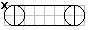
\includegraphics[width=0.3\textwidth]{./inf/SEKII/10_Java_Klassen/raupe_lang.png}
\end{center}

\item Programmiere ein Anwendungsfenster und erzeuge im Anwendungsfenster
mehrere Raupen-Objekte mit unterschiedlichen Attributen und zeichne sie in der
Methode \lstinline|myPaint()|.

\item Erzeuge im Anwendungsfenster ein Objekt der Klasse \myClass{Timer}, damit
die Methode \lstinline|myPaint()| wiederholt aufgerufen wird.

\item Die Raupe soll sich wiederholt von links nach rechts über den Bildschirm
bewegen. Programmiere dazu in der Klasse \myClass{Raupe} eine parameterlose
Methode \lstinline|bewegen()|, die die x-Position der Raupe entsprechend ihrer
Geschwindigkeit nach rechts verschiebt. Nachdem die Raupe aus dem Bild
„gelaufen“ ist, soll ihre neue x-Position so gewählt werden, dass sie langsam
in das Bild hinein gleitet.

Rufe im Anwendungsfenster in der Methode \lstinline|myPaint()| die Methode
\lstinline|bewegen()| für jede Raupe auf.

\item Die Laufbewegung einer Raupe soll auf einfache Weise simuliert werden, in
dem die Raupe ihre Größe verändert.

\begin{compactitem}
\item Leichte Variante: Die Raupe soll immer abwechselnd einmal mit normaler
Länge gezeichnet werden und beim nächsten Mal wie abgebildet verkürzt
dargestellt werden.
\item Schwere Variante: Die Raupe soll immer abwechselnd drei mal hintereinander
mit normaler Länge gezeichnet werden und dann drei mal hintereinander auf
folgende Weise verkürzt dargestellt werden:

\begin{center}
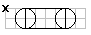
\includegraphics[width=0.32\textwidth]{./inf/SEKII/10_Java_Klassen/raupe_kurz.png}
\end{center}

\end{compactitem}

\end{compactenum}


\subsection{Aufgabe 3: Strichmännchen}

\begin{compactenum}[a)]
\item Überlege dir, welche Attribute die Klasse \myClass{Strichmaennchen}
besitzen muss. Damit es nicht zu langweilig wird, sollen sich die Objekte der
Klasse \myClass{Strichmaennchen} in folgenden Eigenschaften unterscheiden:

\begin{minipage}{0.85\textwidth}
\begin{compactitem}
\item unterschiedliche Kleidung (Farbe)
\item Laufen in unterschiedlichen Geschwindigkeiten
\item unterschiedliche y-Positionen (einige Männchen laufen oben andere weiter
unten)
\end{compactitem}

Ein Strichmännchen soll zunächst zwei Methoden erhalten:

\begin{compactitem}
\item Eine Methode \lstinline|zeichnen()|, die ein Strichmännchen an seiner
aktuellen Position auf dem Bildschirm malt.
\item Eine Methode \lstinline|laufen()|, die ein Strichmännchen entsprechend
seiner aktuellen Geschwindigkeit eine Position nach vorne setzt.
\end{compactitem}
\end{minipage}
\begin{minipage}{0.15\textwidth}
\begin{center}

\includegraphics[width=0.4\textwidth]{./inf/SEKII/10_Java_Klassen/strichmaennchen.png}
\end{center}
\end{minipage}

\item Entwirf die Figur eines Strichmännchens auf kariertem Papier.

\item Programmiere die Klasse \myClass{Strichmaennchen} und erzeuge mehrere
Strichmännchen-Objekte, die über den Bildschirm laufen. Alle Strichmännchen
sollen unterschiedliche Attribut-Werte besitzen. Bei jedem Aufruf der
\lstinline|myPaint()|-Methode werden die Strichmännchen durch Aufruf der
Methode \lstinline|laufen()| um eine Position weiter nach rechts bewegt.
Anschließend werden sie durch Aufruf der Methode \lstinline|zeichnen()| an ihrer
aktuellen Position auf dem Bildschirm gemalt. Verwende die Klasse
\myClass{Timer}, damit die Methode \lstinline|myPaint()| in regelmäßigen
Abständen immer wieder aufgerufen wird.

\item Das Strichmännchen soll jetzt etwas lebendiger gestaltet werden, in dem
es zyklisch in verschiedenen Positionen oder mit verschiedenen Bildern gemalt
wird. Zum Beispiel könnte man vier verschiedene Bilder des Strichmännchens
entwerfen, bei denen die Arme und Beine sich jeweils in unterschiedlichen
Laufstellungen befinden. Wenn man diese Bilder dann der Reihe nach immer
wiederholt, entsteht für den Betrachter der Eindruck einer Bewegung.

\item Vermutlich habt ihr alle ein typisch europäisches Strichmännchen
gezeichnet. Ein großer Teil der Weltbevölkerung besteht aber aus Afrikanern,
Asiaten, usw.. Damit auch diese Personen zu ihrem „Strichmännchen-Recht“
kommen, wird die Klasse \myClass{Strichmaennchen} so abgewandelt, dass jedes
dritte Strichmännchen automatisch mit „fremdländischen“ Attributen versehen
wird, z.B. eine dunklere Hautfarbe. Dazu wird in der Klasse Strichmännchen ein
Zähler benötigt, der als Klassenvariable realisiert wird.
\end{compactenum}


\subsection{Aufgabe 4: Blumen}

\begin{compactenum}[a)]
\item Programmiere in einer neuen Datei eine Klasse \myClass{Blume}.

Eine Blume besitzt zu Anfang die Attribute x-Position, y-Position und Farbe.
Weitere Attribute dürfen später nach Bedarf hinzugefügt werden. Die Startwerte
für die x- und y-Position werden im Konstruktor als Parameter übergeben (in
dieser Reihenfolge). Die Farbe wird automatisch auf rot gestellt.

Schreibe eine Methode \lstinline|zeichnen()|, die die Blume an ihrer aktuellen
Position zeichnet. Das Kreuz markiert die linke obere Ecke, die durch den x-
und y-Wert beschrieben wird (1 Kästchen entspricht 10 Pixeln):

\begin{minipage}{0.5\textwidth}
\begin{center}
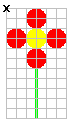
\includegraphics[width=0.2\textwidth]{./inf/SEKII/10_Java_Klassen/blumeBluehend.png}
\end{center}
\end{minipage}
\begin{minipage}{0.5\textwidth}
\begin{center}
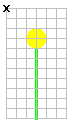
\includegraphics[width=0.2\textwidth]{./inf/SEKII/10_Java_Klassen/blumeVerwelkt.png}
\end{center}
\end{minipage}

Anmerkung: Zu Beginn gibt es nur „blühende“ Blumen (linkes Bild). Die vier
äußeren Kreise werden in der eingestellten Blumen-Farbe ausgefüllt. Der
mittlere Kreis wird gelb gefüllt. Der Stängel wird als ausgefülltes, grünes
Rechteck mit drei Pixel Breite gezeichnet und geht von der Blume bis zum Boden
(also bis zum unteren Rand des Fensters). Der Einfachheit halber kann man den
Stängel auch über den Rand des Fensters hinaus zeichnen.

\item Erzeuge ein Anwendungsfenster mit mindestens sechs Blumen-Objekten. Füge
außerdem in das Anwendungsfenster ein Objekt der Klasse \myClass{Timer} ein.

\item Erweitere die Methode \lstinline|zeichnen()| so, dass die Blume bei jedem
Aufruf um ein Pixel wächst bis sie die y-Position 100 erreicht hat. Das heißt
die y-Position wird immer um ein Pixel nach oben verschoben bis die angegebene
Höhe erreicht ist.

\item Sorge im Konstruktor dafür, dass die Blumen automatisch unterschiedliche
Farben erhalten und zwar immer abwechselnd \lstinline|Color.RED|,
\lstinline|Color.BLUE| oder \lstinline|Color.CYAN|. Die erste und die vierte
Blume müssen also rot werden. Die zweite und die fünfte Blumen werden blau und
die dritte und die sechste Blume werden cyan. Selbstverständlich muss der Code
so geschrieben sein, dass er auch für weitere Blumenobjekte funktioniert.

\item Jede Blume verwelkt zwei Sekunden nachdem sie ihre maximale Höhe erreicht
hat und wird dann wie oben rechts abgebildet gezeichnet.
\end{compactenum}


\subsection{Aufgabe 5: Verhältnis von Klassen und Objekten}

Erkläre die Begriffe Klasse und Objekt anhand der folgenden Worte: Hund, Hasso,
Lassie, Katze, Miezi.


\subsection{Aufgabe 6: Fachbegriffe} 

Finde jeweils das richtige Fachwort.

\bgroup
\def\arraystretch{1.2}
\begin{tabular}{|l|p{65mm}|}
\hline
Festlegung von Namen und Datentyp für eine Variable & \\ \hline
Art einer Variable & \\ \hline
Variable, die im Kopf einer Methode deklariert wird & \\ \hline
Anfangswert für eine Variable setzen & \\ \hline
Wiederholungsanweisung & \\ \hline
Eigenschaft, die ein Objekt einer Klasse beschreibt & \\ \hline
Tätigkeit, die Objekte einer Klasse ausführen können & \\ \hline
\end{tabular}
\egroup


\subsection{Aufgabe 7: Variablendeklaration}

\begin{compactenum}[a)]
\item Wie deklariert man eine Variable in Java?
\item Welches Schlüsselwort muss vor einer Variablendeklaration stehen, wenn
eine Variable \ldots 

\bgroup
\def\arraystretch{1.2}
\begin{tabular}{|l|p{45mm}|}
\hline
\ldots nicht verändert werden darf (also konstant ist) & \\ \hline
\ldots von einer anderen Klasse benutzt werden darf. & \\ \hline
\ldots von einer anderen Klasse nicht benutzt werden darf. & \\ \hline
\ldots nur einmal pro Klasse vorhanden ist (also nicht für jedes Objekt). & 
\\ \hline
\end{tabular}
\egroup
\end{compactenum}


\subsection{Aufgabe 8: Entwurf einer Methode (1)}

Programmiere auf Papier eine Methode \lstinline|treffer()|, die eine
Fließkommazahl als Parameter erhält und einen booleschen Wert zurück gibt. Es
wird der Wert \lstinline|true| zurückgegeben, wenn eine der Zahlen
\lstinline|1.5|, \lstinline|4| oder \lstinline|5.5| angegeben wird. Andernfalls
wird der Wert \lstinline|false| zurück gegeben.


\subsection{Aufgabe 9: Entwurf einer Methode (2)}

Programmiere auf Papier eine Methode \lstinline|summe()|, die eine ganze Zahl
\lstinline|x| als Parameter erhält und eine (eventuell sehr große) ganze Zahl
als Rückgabewert zurück gibt. Die Methode soll alle ganzen Zahlen von zehn bis zu
der übergebenen Zahl \lstinline|x| aufaddieren.


\subsection{Aufgabe 10: Programmierung von Klassen und Objekten}

\begin{compactenum}[a)]
\item Mit welchem Schlüsselwort kennzeichnet man beim Programmieren eine
Klasse?
\item Angenommen es existiert eine Klasse \myClass{Fisch}. Wie erzeugt man im
Anwendungsfenster eine Variable, die auf ein Objekt dieser Klasse verweisen
kann?
\item Wie erzeugt man ein neues Objekt der Klasse im Speicher?
\item Wann wird das Objekt wieder aus dem Speicher gelöscht?
\end{compactenum}


\subsection{Aufgabe 11: Verweis auf sich selbst}

Eine Klasse beschreibt das Schema für eine ganze Gruppe von Objekten. Wie
verweist man beim Programmieren innerhalb der Klasse auf das eigene Objekt
(also quasi auf sich selber)? 


\subsection{Aufgabe 12: Konstruktor}

\begin{compactenum}[a)]
\item Was ist ein Konstruktor?
\item Wann wird der Konstruktor einer Klasse aufgerufen?
\item Wie programmiert man einen Konstruktor?
\end{compactenum}


\subsection{Aufgabe 13: Leseübung}

Lies den folgenden Programmtext sorgfältig und beantworte die unten gestellten
Fragen.

\begin{lstlisting}
class Demo {
  public String name = "Demo";
  public double gewicht = 55.5;
  public int groesse;
  public static int alter;

  public Demo(String name, double gewicht) {
    this.name = name;
    gewicht = 87.2;
    alter = 50;
  }

  public Demo(String name, int a) {
    this.name = name;
    groesse = 183;
    alter = a;
  }

  public void drucken() {
    // Ausgabe der Daten eines Objektes auf die Konsole
    System.out.println("Name: "+name);
    System.out.println("Gewicht: "+gewicht);
    System.out.println("Groesse: "+groesse);
    System.out.println("Alter: "+alter);
    System.out.println(" ---");
  }

  public static void main(final String[] args) {
    Demo a = new Demo("Mona", 51.3);
    Demo b;
    Demo c = a;
    Demo d = new Demo ("Simson", 19);
    c.gewicht = 45.0;
    a.drucken();
    c.drucken();
    d.drucken();
  }
}
\end{lstlisting}

\begin{compactenum}[a)]
\item Markiere im Code die Deklaration einer Klassenvariablen (K), einer
Objektvariablen (O) und einer lokalen Variablen (L).
\item Welche Methoden können benutzt werden, ohne dass es ein Objekt gibt?
\item Ermittle, welche Ausgabe das folgende Programm erzeugt. Zeichne dazu den
Inhalt der Objekte und Variablen im Hauptspeicher auf, um den Ablauf des
Programms nachzuvollziehen.
\item Was passiert wenn man \lstinline|b.drucken();| aufruft?
\item Was passiert bei der Anweisung: \lstinline|b = new Demo();| ?
\end{compactenum}

Hinweis: Du findest die Datei \myFile{Demo.java} im Kurs-Repository. Du solltest
die Aufgaben aber zunächst wirklich beantworten, ohne das Programm in Eclipse
auszuführen. Das kannst du dann anschließend tun um deine eigenen Antworten zu
überprüfen.


\subsection{Aufgabe 14: Autorennen}

\begin{compactenum}[a)]
\item Programmiere in einer neuen Datei eine Klasse \myClass{Auto}.

\item Ein Auto besitzt zu Beginn die Attribute x-Position, y-Position und
Farbe. Weitere Attribute dürfen später nach Bedarf hinzugefügt werden. Die
Startwerte für den y-Wert und die Farbe werden im Konstruktor als Parameter
übergeben (in der angegebenen Reihenfolge). Die x-Position wird automatisch auf
den Wert 10 gesetzt.

Schreibe eine Methode \lstinline|zeichnen()| (mit dem \myClass{Graphics}-Objekt
als Parameter), die das Auto an seiner aktuellen Position wie abgebildet
zeichnet. Zunächst werden zwei große ausgefüllte Rechtecke in der eingestellten
Autofarbe gezeichnet. Anschließend werden die Fenster mit zwei ausgefüllten
gelben Quadraten darüber gemalt. Danach wird der Bereich für den Auspuff und
die Räder schwarz ausgefüllt. Das Kreuz markiert die linke obere Ecke, die durch
den x- und y-Wert beschrieben wird. Ein Kästchen in der Abbildung entspricht
zehn Pixeln:

\begin{center}
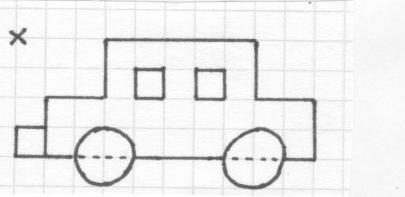
\includegraphics[width=0.25\textwidth]{./inf/SEKII/10_Java_Klassen/auto.jpg}
\end{center}

\item Erzeuge ein Anwendungsfenster mit einer Breite von 800 Pixeln und einer
Höhe von 500 Pixeln. Zeichne im Anwendungsfenster mehrere Objekte der Klasse
\myClass{Auto}. Füge auch ein Objekt der Klasse \myClass{Timer} ein, das die
\lstinline|myPaint()|-Methode im Abstand von 100 Millisekunden wiederholt
aufruft.

\item Die Autos sollen sich nun bewegen. Füge dazu ein Attribut
\lstinline|speed| mit dem Datentyp \lstinline|int| in die Klasse ein, und setze
das Attribut im Konstruktor auf einen Zufallswert zwischen 5 und 14.

Um Zufallswerte erzeugen zu können, musst du in die Klasse \myClass{Auto} auch
noch eine Objekt der Klasse \myClass{Random} einfügen. Beachte, dass dieses
Objekt eine Klassenvariable sein muss, denn wenn jedes Auto seinen eigenen
Zufallsgenerator hätte, würden die meisten Autos exakt dieselbe Geschwindigkeit
erhalten, weil ihr Zufallsgenerator jeweils mit dem selben Anfangswert gestartet
wird.

Erweitere anschließend die Methode \lstinline|zeichnen()| so, dass die
x-Position des Autos bei jedem Aufruf um den Wert \lstinline|speed| nach rechts
verschoben wird. Wenn die x-Position größer als 800 ist, soll seine x- Position
links vor das Fenster gesetzt werden, so dass das Auto langsam in das Fenster
hinein gleitet.

\item Die Abgase des Autos sollen mit grau ausgefüllten Kreisen animiert
werden. Dazu werden vier Zustände unterschieden (durchnummeriert von 0 bis 3),
die das Auto der Reihe nach wiederholt durchläuft. Im Zustand 0 werden
keinerlei Abgase gezeichnet. Im Zustand 1 wird nur der mit 1 bezeichnete Kreis
gezeichnet. Im Zustand 2 werden die mit 1 und 2 bezeichneten Kreise gezeichnet.
Im Zustand drei werden alle drei Kreise gezeichnet.

\begin{center}
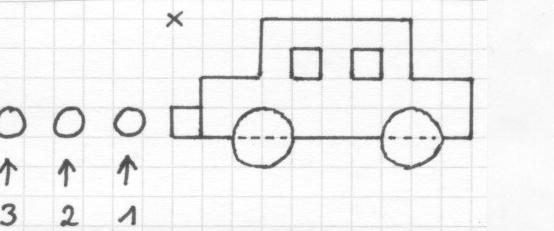
\includegraphics[width=0.3\textwidth]{./inf/SEKII/10_Java_Klassen/autoMitAbgasen.jpg}
\end{center}

\item Die Autos sollen in der Reihenfolge ihrer Erzeugung durchnummeriert
werden. Das erste Auto erhält die Nummer 1. Dazu musst du eine Klassenvariable
erzeugen, mit der die Autos im Konstruktor durchgezählt werden. Außerdem
benötigt man eine Objektvariable, in der jedes Auto seine eigene Nummer
abspeichert.

In der Methode \lstinline|zeichnen()| soll jedes Auto seine Nummer mit der
\myClass{Graphics}-Methode \lstinline|drawString()| an der Position (x+50, y+35)
mit schwarzer Schrift ausgeben.

\item Ein Autorennen dauert drei Runden. Nachdem ein Auto dreimal von links nach
rechts durch das Fenster gefahren ist, soll es nicht mehr gezeichnet werden.

Außerdem soll die Nummer des Autos, das als erstes „das Ziel“ erreicht, im
Anwendungsfenster an der Position (300, 480) mit einem kleinen Text ausgegeben
werden, z.B. „\myUserInput{Der Sieger ist Auto 4}“. Welche Klasse diese Ausgabe
übernimmt, darfst du selber entscheiden.
\end{compactenum}


\subsection{Aufgabe 15: Sternen-Himmel}

Es soll ein Sternen-Himmel programmiert werden.

\begin{compactenum}[a)]
\item Wähle im Anwendungsfenster-Fenster die Farbe schwarz als
Hintergrundfarbe aus.

\item Programmiere eine Klasse \myClass{Stern} mit folgenden Attributen:

\begin{compactitem}
\item der Farbe des Sterns
\item der linken oberen Ecke des Sterns (x- und y-Position)
\item der Geschwindigkeit des Sterns (Veränderung der x-Richtung in Pixel pro
Aufruf vom \lstinline|myPaint()|)
\end{compactitem}

Alle Attribute der Klasse dürfen von außen (d.h.\ von einer anderen Klasse aus)
nicht verändert werden. Weise den Variablen in der Klasse die entsprechende
Eigenschaft zu. Zur Programmierung der im nachfolgenden beschriebenen
Funktionalitäten dürfen weitere Klassen- und Instanzvariablen eingefügt werden.
Auch diese Variablen dürfen jedoch nicht von außen veränderbar sein.

Die Klasse Stern soll nur einen einzigen Konstruktor haben, in dem als
Parameter die x- und y- Position der linken oberen Ecke des Sterns angegeben
werden. Die Geschwindigkeit wird innerhalb des Konstruktors automatisch für
alle Sterne auf den Wert 3 gesetzt. Auch die Farbe wird automatisch generiert.
Jeder zweite Stern erhält die Farbe orange. Alle anderen Sterne erhalten die
Farbe gelb.

\vspace{1mm}

\begin{minipage}{0.85\textwidth}
Die Klasse Stern besitzt die öffentliche Methode \lstinline|zeichnen()|, die den
Stern an seiner aktuellen Position malt und ihn anschließend entsprechend der
eingestellten Geschwindigkeit in der x-Position verschiebt. Entscheide selbst, ob
die Methode \lstinline|zeichnen()| einen Parameter benötigt oder nicht. Ein
Stern wird durch zwei ausgefüllte Dreiecke gemalt, wie in der nebenstehenden
Abbildung zu sehen ist. Die linke obere Ecke, die durch die x- und y-Werte
beschrieben ist, ist im Bild durch einen dicken Punkt markiert. Dieser Punkt
soll natürlich nicht mit gezeichnet werden. Wähle beim Zeichnen pro Kästchen
eine Größe von 10 Pixel. Wenn ein Stern rechts aus dem Bild gewandert ist, soll
die Methode \lstinline|zeichnen()| ihn wieder auf der linken Seite ins Bild
setzen.
\end{minipage}
\begin{minipage}{0.15\textwidth}
\begin{center}
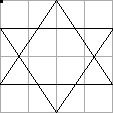
\includegraphics[width=0.5\textwidth]{./inf/SEKII/10_Java_Klassen/stern.png}
\end{center}
\end{minipage}

\vspace{1mm}

Damit ein Stern harmonisch in das Bild hinein gleitet, wird seine neue
x-Position nicht auf den Wert 0 gesetzt, sondern soweit nach links verschoben,
das zunächst nur seine rechten Spitzen sichtbar sind.

\item Erzeuge im Anwendungsfenster mindestens vier verschiedene Objekte der
Klasse \myClass{Stern} an verschiedenen Positionen. Sorge mit Hilfe der Klasse
\myClass{Timer} dafür, dass das Anwendungsfenster und die Sterne alle 100
Millisekunden neu gezeichnet werden.

\item Die Klasse \myClass{Stern} soll um das boolesche Attribut
\lstinline|blinkend| erweitert werden. Auch dieses Attribut darf von außen nicht
verändert werden. Der Standard-Wert für das Attribut ist \lstinline|false|
(ausgeschaltet).

Füge in die Klasse einen zweiten Konstruktor ein, mit dem neben der x- und
y-Position der Wert des Attributs \lstinline|blinkend| eingestellt werden kann.
Wenn \lstinline|blinkend| auf \lstinline|true| gesetzt wird, wird das Objekt nur
bei jedem zweiten Aufruf der Methode \lstinline|zeichnen()| tatsächlich
gezeichnet, so dass ein Blink-Effekt entsteht. 

Erzeuge im Anwendungsfenster ein weiteres Objekt der Klasse \myClass{Stern}, bei
dem das Attribut \lstinline|blinkend| eingeschaltet ist.

\item Hin und wieder ziehen am Himmel Wolken vorbei und verdecken die Sterne.
Wenn eine Wolke da ist, sind alle Sterne nicht sichtbar und werden daher nicht
gezeichnet. Ergänze die Klasse \myClass{Stern} um ein öffentliches boolesches
Attribut \lstinline|wolke_da|, das nur einmal für die gesamte Klasse existieren
soll.
Wenn eine Wolke vorhanden ist, werden die Sterne in der Methode
\lstinline|zeichnen()| nicht gezeichnet. Achte darauf, dass der Wolken-Effekt
auch für blinkende Sterne korrekt funktioniert.

Stelle das boolesche Attribut \lstinline|wolke_da| des Anwendungsfensters so
ein, dass immer abwechselnd 1200 ms lang keine Wolke da ist und dann 600 ms
lang eine Wolke vorüber zieht.
\end{compactenum}


\subsection{Aufgabe 16: Bälle (alte Klausuraufgabe)}

\emph{Hinweis: In kursiver Schrift wird bei einigen Teilaufgaben eine
Alternative für diejenigen vorgeschlagen, die Probleme haben, die Teilaufgabe
zu lösen. Der Alternativ-Vorschlag soll euch dazu befähigen, mit den anderen
Teilaufgaben weiterzumachen, damit ihr euch nicht an einem Problem fest beißt.
Wer den Alternativ- Vorschlag wählt, erhält für die jeweilige Teilaufgabe
natürlich nicht die volle Punktzahl.}

\begin{compactenum}[a)]
\item Erzeuge ein Anwendungsfenster mit einem schwarzen Hintergrund und weißer
Vordergrundfarbe. Das Anwendungsfenster soll eine Breite und Höhe von je 500
Pixel besitzen.

\item Programmiere in einer zweiten Datei eine Klasse \myClass{Ball}. Alle
Attribute der Klasse \myClass{Ball} sollen vor dem Zugriff von außen (d.h.\ vom
Anwendungsfenster aus) geschützt sein. Alle Methoden sind öffentlich und dürfen
vom Anwendungsfenster aus benutzt werden.

Ein Ball besitzt zu Anfang die Attribute x-Position, y-Position, Breite und
Farbe. Weitere Attribute dürfen später nach Bedarf hinzugefügt werden. Die
x-Position wird automatisch auf den Wert 25 festgelegt, die y-Position auf den
Wert 250 und die Breite auf den Wert 50. Nur die Farbe kann vom
Anwendungsfenster aus eingestellt werden und wird im Konstruktor als Parameter
übergeben.

Schreibe eine Methode \lstinline|zeichnen()|, die den Ball an seiner aktuellen
Position und in der für ihn gewählten Farbe als ausgefüllten Kreis zeichnet.
Entscheide selbst welche Parameter und welchen Rückgabewert die Methode
\lstinline|zeichnen()| benötigt.

\item Erzeuge im Anwendungsfenster ein Objekt der Klasse \myClass{Ball}, das
eine rote Farbe besitzt.

\item Füge im Anwendungsfenster ein Objekt der Klasse \myClass{Timer} ein, und
stelle den Timer so ein, dass die \lstinline|myPaint()|-Methode alle zehn
Millisekunden aufgerufen wird.

\item Erweitere in der Klasse \myClass{Ball} die Methode \lstinline|zeichnen()|,
so dass in der Methode die x-Position des Balls bei jedem Aufruf um zwei Pixel
verschoben wird. Der Ball soll immer abwechselnd zunächst nach rechts rollen
bis zur x-Position 425 und anschließend wieder zurück nach links bis zur
x-Position 25.

\emph{Falls es dir nicht gelingt den Ball abwechselnd nach rechts und wieder
nach links zu steuern, versuche den Ball -- wie das Strichmännchen -- immer von
links nach rechts rollen zu lassen. Das heißt, das der Ball nach Erreichen der
x-Position 425 wieder auf die x-Position 25 gesetzt wird. (halbe Punktzahl)} 

\item Erweitere die Klasse \myClass{Ball} so, dass jedes weitere Ball-Objekt
automatisch in seiner anfänglichen x- Position um 50 Pixel nach rechts
verschoben wird. Das erste Ball-Objekt besitzt bei Erzeugung die x- Position
25, das zweite Ball-Objekt die x-Position 75, das dritte Ball-Objekt die
x-Position 125, usw.

Erzeuge im Frame acht verschiedene Ball-Objekte, die unterschiedliche Farben
besitzen sollen. Die Farben darfst du frei wählen. Wenn du alles richtig
gemacht hast, bilden die Ball-Objekte eine Art „Schlange“.

\emph{Falls dir die Lösung dieser Aufgabe nicht gelingt, überspringe die Aufgabe
und arbeite einfach mit einem Ball-Objekt weiter.}

\item Die Klasse \myClass{Ball} soll so erweitert werden, dass sich der Ball im
Uhrzeigersinn im Kreis bewegt. Wenn der Ball sich nach rechts bewegt, wird die
y-Koordinate in Abhängigkeit von der x-Koordinate folgendermaßen berechnet:

\begin{lstlisting}
y = 250 - (int) Math.sqrt(40000-(x-225)*(x-225));
\end{lstlisting}

Dadurch bewegt sich der Ball im Halbkreis nach oben. Wenn sich der Ball nach
links bewegt, wird die y- Koordinate mit der Formel

\begin{lstlisting}
y = 250 + (int) Math.sqrt(40000-(x-225)*(x-225));
\end{lstlisting}

berechnet. Dadurch bewegt sich der Ball im Halbkreis nach unten. Beachte, dass
der Ball bei dieser Technik an den Seiten links und rechts wesentlich schneller
rollt als in der Mitte. Das ist kein Programmierfehler.

Vorgabe: Berechne die y-Koordinate für den Ball mit Hilfe einer Methode, die
die x-Koordinate als Parameter erhält und die y-Koordinate als Rückgabewert
zurück gibt. Schreibe entweder für jede der beiden Formeln eine Methode oder
programmiere eine einzige Methode, die die aktuelle Richtung des Balls
berücksichtigt.

\emph{Falls du nicht weißt, wie man die Methode programmiert, löse die Aufgabe
ohne Verwendung einer neuen Methode. (halbe Punktzahl)}

\item Erweitere die Klasse \myClass{Ball} so, dass ein Ball zyklisch immer
zweimal im Kreis rollt und dann einmal wie in Teilaufgabe (e) mit fester
y-Koordinate nach rechts und wieder zurück nach links rollt. Das heißt, die
Berechnung der y-Koordinate mit den Kreis-Formeln entfällt bei jedem dritten
Durchgang.
\end{compactenum}